\documentclass[10pt]{article}
\usepackage[margin=0.75in]{geometry}
\usepackage[T1]{fontenc}
\usepackage{lmodern}
\usepackage{graphicx,booktabs}
\usepackage[colorlinks=true,urlcolor=blue]{hyperref}
\setlength{\parindent}{0pt}
\setlength{\parskip}{5pt}
\begin{document}
\begin{center}
{\Large\bfseries Lab 3: MLP Experiments on Sonar}\\[3pt]
COMP 395 \quad | \quad charliewu0788
\end{center}

\textbf{Design.} All models used the supplied split: 166 training examples and 42 validation examples, with 60 features standardized using training statistics. The five MLPs used a sigmoid output, binary cross-entropy (BCE), learning rate 0.001, 100 epochs, batch size 1, and seed 0. Relative to the 32-unit ReLU/Adam model, each variant changed one factor: activation, width, depth, or optimizer. Adam and SGD otherwise used their defaults. The linear baseline used its supplied MSE/SGD setup. The Random Forest used 200 trees and \texttt{random\_state=0}, with other settings at their defaults.

\begin{center}
\small
\begin{tabular}{lrr}
\toprule
Model (hidden layers / optimizer) & Train accuracy & Validation accuracy \\
\midrule
Linear baseline & 94.58\% & 80.95\% \\
ReLU 32 / Adam & 100.00\% & \textbf{92.86\%} \\
Tanh 32 / Adam & 100.00\% & 83.33\% \\
ReLU 64 / Adam & 100.00\% & 88.10\% \\
ReLU 32, 16 / Adam & 100.00\% & \textbf{92.86\%} \\
ReLU 32 / SGD & 98.19\% & 90.48\% \\
Random Forest (200 trees) & 100.00\% & 85.71\% \\
\bottomrule
\end{tabular}
\end{center}

\textbf{Learning curves.} Figure 1 overlays the same five MLPs in both panels; all losses are BCE, so their scales are comparable. The deeper ReLU model learned fastest: training loss fell below 0.1 at logged epoch 6, versus 9 for ReLU 32/Adam and 16 for Tanh. At epoch 10, the deeper model's training loss was 0.0118, compared with 0.0868 for ReLU 32/Adam. SGD was slower, ending at 0.1293, but its loss kept falling; it was not stuck. These are convergence comparisons at the chosen learning rate, not a claim that Adam always beats SGD.

\textbf{Overfitting.} The Adam models fit the training data perfectly, but validation loss eventually increased. Tanh showed the clearest case: validation BCE reached 0.3968 at epoch 10 and rose to 1.2388 by epoch 99. ReLU 64 also rose from 0.2140 at epoch 15 to 0.5590. The deeper model rose from 0.1120 at epoch 10 to 0.3471, despite retaining high final accuracy. This suggests increasingly confident errors; accuracy alone hides that behavior. SGD's final validation loss, 0.2832, was also its minimum over the run. Epoch indices in the plots run from 0 to 99.

\textbf{Comparison.} The best MLPs classified 39/42 examples correctly, versus 36/42 for the forest and 34/42 for the linear baseline. Learned nonlinear features may suit this split better than the forest's axis-aligned splits, but this is a hypothesis. Extra width did not help, and extra depth tied the smaller model, so ReLU 32/Adam is the simpler best choice (1,985 versus 2,497 parameters). One validation example changes accuracy by 2.38 percentage points; one seed and one split do not establish a general winner. The held-out split was used for model comparison, not an independent final test.

\small
\textbf{W\&B project:} \href{https://wandb.ai/charl1e88-occidental-college/comp395-lab3-sonar}{charl1e88-occidental-college / comp395-lab3-sonar}.\\
\textbf{AI assistance:} Code implementation, experiment execution, and report drafting were assisted by Codex.

\newpage
\begin{center}
{\large\bfseries W\&B experiment curves}\\[8pt]
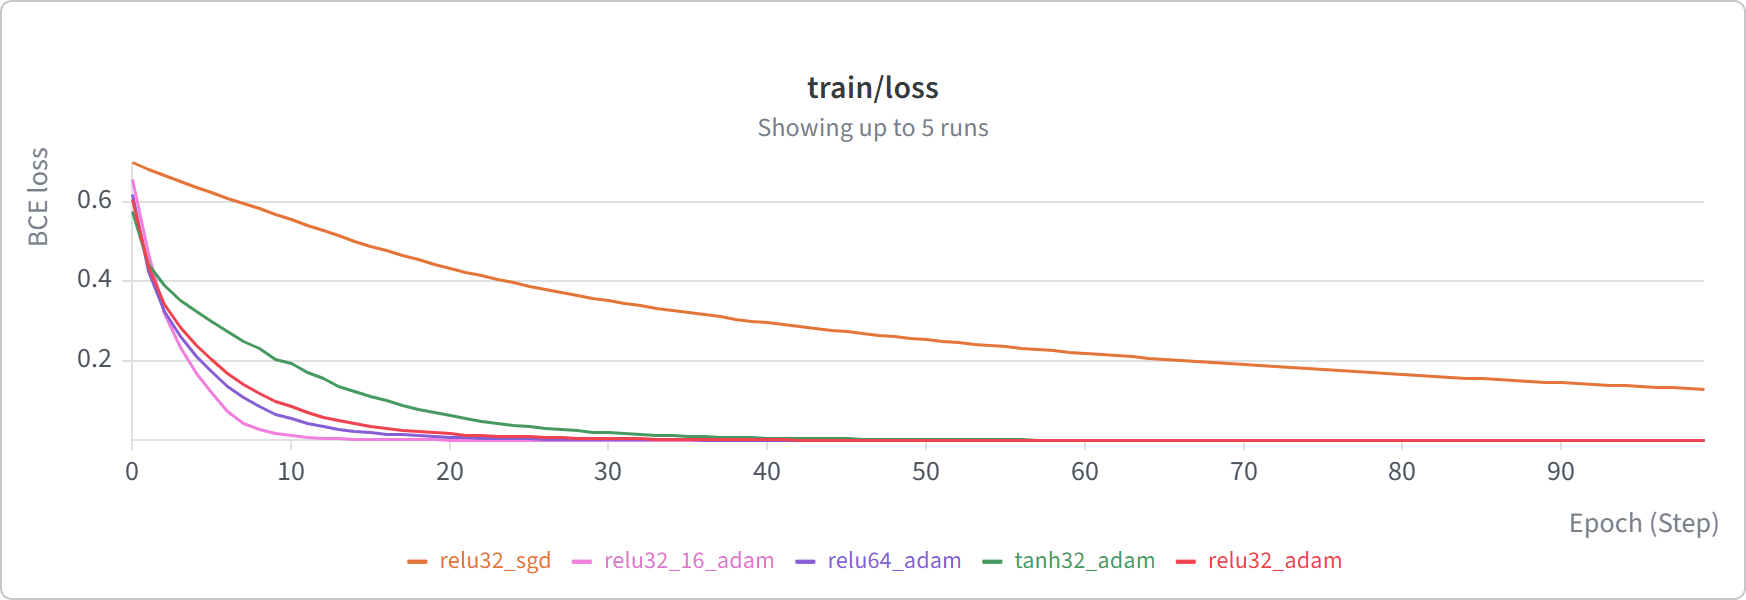
\includegraphics[width=\textwidth]{wandb_train_loss.png}\\[10pt]
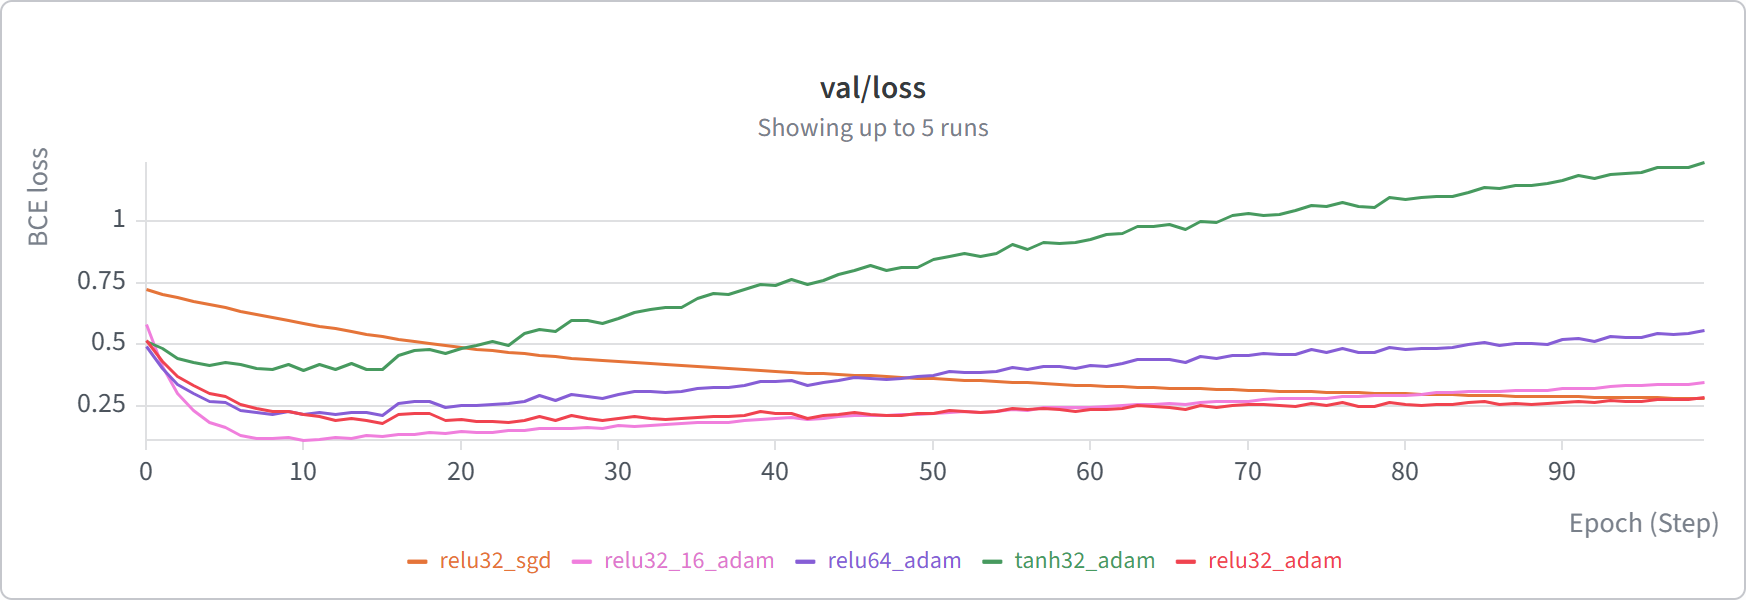
\includegraphics[width=\textwidth]{wandb_val_loss.png}
\end{center}
\textbf{Figure 1.} W\&B panels for training BCE (top) and validation BCE (bottom), overlaying the five MLP runs with no smoothing. Both panels use logged epoch (\texttt{Step}, 0--99). These images were captured from W\&B, not plotted separately in matplotlib. The linear baseline is excluded because it uses MSE rather than BCE; the forest does not have an epoch-wise loss curve.
\end{document}
